\documentclass[a4paper, 11pt]{article}
\usepackage[slovak]{babel}
\usepackage[utf8]{inputenc}
\usepackage{fullpage}
\usepackage{float}
\usepackage{graphicx}
\usepackage{subcaption}

\title{Model domovov dôchodcov}

\begin{document}
\begin{center}
\Large \textbf{ESP8266: snímání teploty}(28)
\end{center}
\noindent
\today \hfill \textbf{Martin Bažík}, xbazik00 \\

\section{Úvod}
Tento projekt je zameraný na vytvorenie WiFi AP (bod pripojenia) na module WeMos ESP8266, ktorý vďaka teplotnému čidlu DS18B20 poskytuje informácie o súčasnej teplote a starých meraniach. Pre komunikáciu s týmto AP bola vytvorená Android aplikácia Thermometer. 

\section{Popis ovládania}
Užívateľ sa pripojí na AP ES\_29D9AE a zapne aplikáciu Thermometer. Po zapnutí aplikácie stlačí tlačidlo \texttt{READ TEMPERATURE} a zobrazí sa mu aktuálna teplota a zoznam historických meraní. Na tejto obrazovke je monžné stlačením tlačidla \texttt{READ TEMPERATURE} získať nové dáta.
\begin{figure}[H]
\centering
\begin{subfigure}{.5\textwidth}
  \centering
  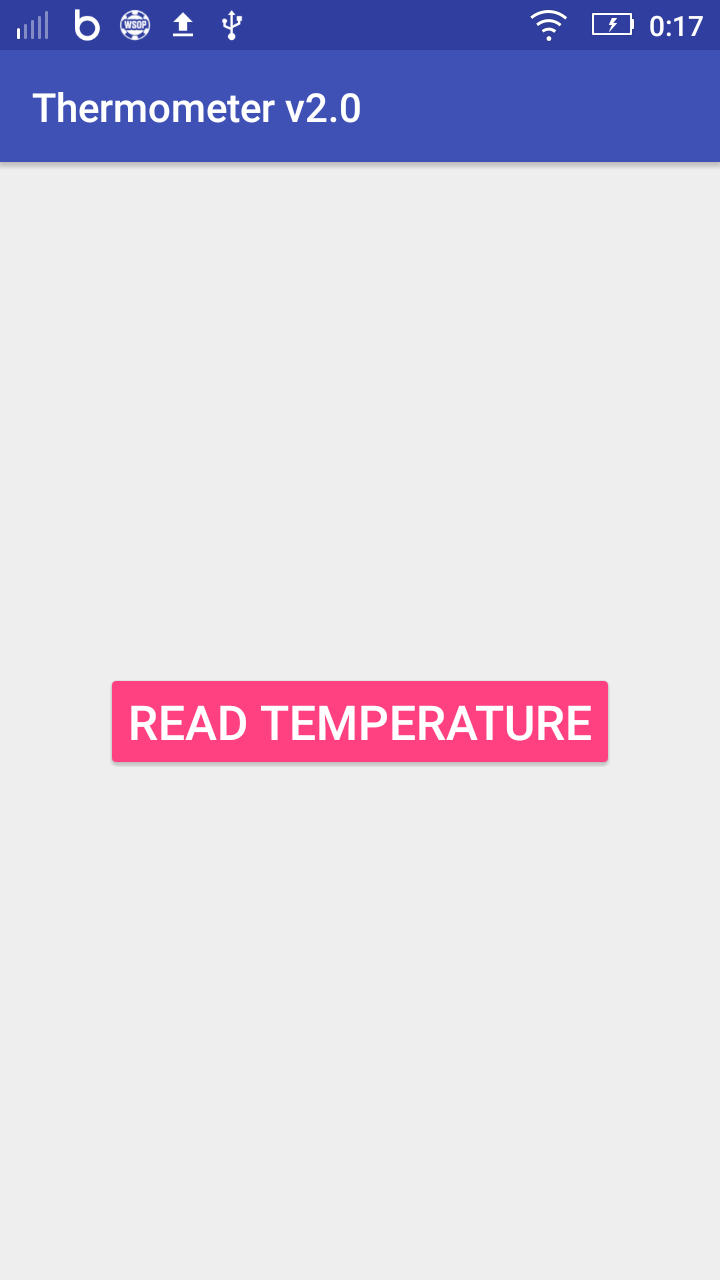
\includegraphics[width=.5\linewidth]{img/app1.png}
  \caption{Počiatočná obrazovka}
  \label{fig:sub1}
\end{subfigure}%
\begin{subfigure}{.5\textwidth}
  \centering
  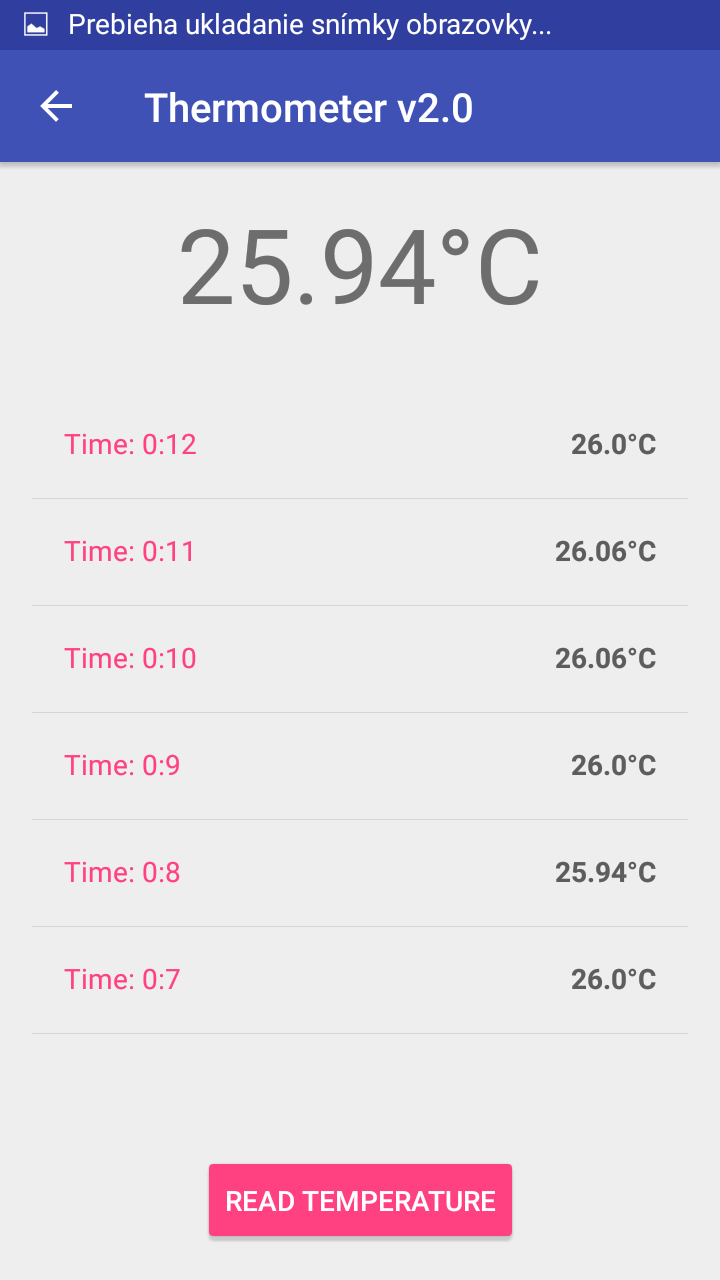
\includegraphics[width=.5\linewidth]{img/app2.png}
  \caption{Obrazovka s hodnotami}
  \label{fig:sub2}
\end{subfigure}
\caption{GUI}
\label{fig:test}
\end{figure}

\section{Schéma zapojenia}
\begin{figure}[H]
	\centering
	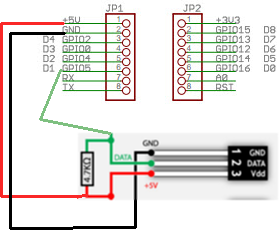
\includegraphics[scale=0.5]{img/scheme.png}
	\caption{Schéma zapojenia}
\end{figure}

\section{Implementácia}
Modul ESP8266 bol naprogramovaný v prostredí arduino. Na module beží HTTP server (knižnica \texttt{ESP8266WebServer}), ktorý vráti informácie o aktuálnej teplote, histórii meraní a súčasnú časovú značku. História meraní je uložená EEPROM (knižnica \texttt{EEPROM}) pamäti, z ktorej sa používa iba priestor na uloženie 10 hodnôt. Teploty sa do nej ukladajú každú minútu a v prípade, že sa naplní najstaršia hodnota sa odstráni a na najvyššiu adresu sa uloží súčasná hodnota. 

Tento server je po pripojení na AP ES\_29D9AE (knižnica \texttt{ESP8266WiFi}) dostupný na IP adrese \texttt{http://192.168.4.1/}. Server vracia namerané hodnoty vo formáte JSON.

Teplota je meraná pomocou knižnice \texttt{OneWire} a interpretovaná využitím knižnice \texttt{DallasTemperature}.

Ako front-end aplikácie bola využitá už spomínaná Android aplikácia Thermometer. Táto aplikácia využíva HTTP požiadavky \texttt{GET} a spracuje JSON. Súčasná teplota je vizualizovaná textom a história pomocou zoznamu. 

\section{Záver}
Server funguje aj po dlhšom behu bez problémov. Nastavenia WiFi AP má pôvodné nastavenia a pripája sa bez hesla. JSON formát nie je vždy validný, lebo obsahuje hodnotu nan v kolekcii float hodnôt. Server má problém spracovať veľkým množstvom požiadavkov.  

\end{document}